\problemname{Klockan}
Timla åkte hemifrån vid midnatt och kom hem nästa midnatt, 24 timmar senare. Då hade det varit inbrott i huset! 
I huset har Timla en digital klocka som visar tiden i 24-timmarsformat med timmar, minuter och sekunder, alltid sex siffror. Timla gillar att spara el, så hennes klocka stänger av sig automatiskt när ingen är i huset. För att kunna mäta exakt hur mycket el hon sparar har hon också en mycket exakt elmätare. Enligt denna mätare förbrukade klockan $N$ energienheter under dygnet då hon var bortrest. Varje siffersegment i klockan drar en energienhet för varje sekund som det siffersegmentet lyser. Siffrorna ser ut som på bilden. Exempelvis lyser 27 siffersegment då klockan är 02:41:35.

\begin{center}
  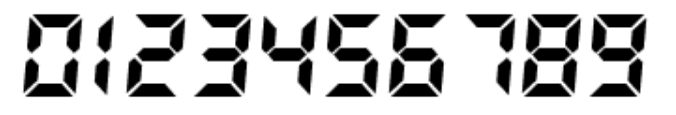
\includegraphics[width=12cm]{illustration.pdf}
\end{center}

Timla vill hjälpa polisen genom att ta reda på vilken tid tjuven kan ha brutit sig in i huset. Man kan se på skoavtrycken att tjuven gick in i huset en gång och ut en gång, så klockan kan inte ha tänts och släckts flera gånger. Klockans display tänds och släcks alltid vid en hel sekund och kan som tidigast ha tänts 00:00:00 och kan som senast ha slocknat efter att ha visat 23:59:59. För givna $N$ finns minst ett tidsintervall under dygnet då klockan förbrukar $N$ energienheter.

Skriv ett program som beräknar antalet möjliga klockslag då displayen kan ha tänts. 

\section*{Indata}
Ett positivt heltal $n$. För givna $n$ finns minst ett tidsintervall under dygnet då klockan förbrukar $n$ energienheter.

\section*{Utdata}
Skriv ut ett tal: antalet olika klockslag då klockans display kan ha tänts. 

\section*{Poängsättning}
Din lösning kommer att testas på fem olika testfall.

\noindent
\begin{tabular}{| l | l | l |}
  \hline
  Fall & Poängvärde & Gränser \\ \hline
  $1$    & $20$        &  $n \le 23$ \\ \hline 
  $2$    & $20$        &  $n \le 200$ \\ \hline 
  $3$    & $20$        &  Inga ytterligare begränsningar. \\ \hline
  $4$    & $20$        &  Inga ytterligare begränsningar. \\ \hline
  $5$    & $20$        &  Inga ytterligare begränsningar. \\ \hline
\end{tabular}

\section*{Poängsättning}
För 1 poäng gäller att $n \le 23$. \\
För ytterligare 1 poäng gäller att $n \le 200$.

\section*{Förklaring av exempel}
I det första exemplet måste klockan ha varit igång i exakt en sekund. Det kan ha varit under 11:11:17, 11:17:11 eller 17:11:11.

I det andra exemplet är den enda möjligheten att klockan var på hela dygnet, från 00:00:00 till och med 23:59:59.

I det tredje exemplet finns 3196 möjligheter för när klockan kan ha startat. Exempelvis kan den ha startat 20:02:06 och slocknat efter att ha visat 20:02:08.
